\documentclass[a4paper,11.5pt]{article}
\usepackage[textwidth=170mm, textheight=230mm, inner=20mm, top=20mm, bottom=30mm]{geometry}
\usepackage[normalem]{ulem}
\usepackage[utf8]{inputenc}
\usepackage[T1]{fontenc}
\PassOptionsToPackage{defaults=hu-min}{magyar.ldf}
\usepackage[magyar]{babel}
\usepackage{amsmath, amsthm,amssymb,paralist,array, ellipsis, graphicx,float}
%\usepackage{marvosym}

\makeatletter
\renewcommand*{\mathellipsis}{%
	\mathinner{%
		\kern\ellipsisbeforegap%
		{\ldotp}\kern\ellipsisgap%
		{\ldotp}\kern\ellipsisgap%
		{\ldotp}\kern\ellipsisaftergap%
	}%
}
\renewcommand*{\dotsb@}{%
	\mathinner{%
		\kern\ellipsisbeforegap%
		{\cdotp}\kern\ellipsisgap%
		{\cdotp}\kern\ellipsisgap%
		{\cdotp}\kern\ellipsisaftergap%
	}%
}
\renewcommand*{\@cdots}{%
	\mathinner{%
		\kern\ellipsisbeforegap%
		{\cdotp}\kern\ellipsisgap%
		{\cdotp}\kern\ellipsisgap%
		{\cdotp}\kern\ellipsisaftergap%
	}%
}
\renewcommand*{\ellipsis@default}{%
	\ellipsis@before
	\kern\ellipsisbeforegap
	.\kern\ellipsisgap
	.\kern\ellipsisgap
	.\kern\ellipsisgap
	\ellipsis@after\relax}
\renewcommand*{\ellipsis@centered}{%
	\ellipsis@before
	\kern\ellipsisbeforegap
	.\kern\ellipsisgap
	.\kern\ellipsisgap
	.\kern\ellipsisaftergap
	\ellipsis@after\relax}
\AtBeginDocument{%
	\DeclareRobustCommand*{\dots}{%
		\ifmmode\@xp\mdots@\else\@xp\textellipsis\fi}}
\def\ellipsisgap{.1em}
\def\ellipsisbeforegap{.05em}
\def\ellipsisaftergap{.05em}
\makeatother

\usepackage{hyperref}
\hypersetup{
	colorlinks = true	
}

\begin{document}
	%%%%%%%%%%%RÖVIDÍTÉSEK%%%%%%%%%%
	\setlength\parindent{0pt}
	\def\s{\hspace{0.2mm}\vphantom{\beta}}
	\def\Z{\mathbb{Z}}
	\def\Q{\mathbb{Q}}
	\def\R{\mathbb{R}}
	\def\C{\mathbb{C}}
	\def\N{\mathbb{N}}
	\def\Ra{\overline{\mathbb{R}}}
	
	\def\sume{\displaystyle\sum_{n=1}^{+\infty}}
	\def\sumn{\displaystyle\sum_{n=0}^{+\infty}}
	
	\def\narrow{\underset{n\rightarrow+\infty}{\longrightarrow}}
	\def\limn{\displaystyle\lim_{n\to +\infty}}
	\def\limx{\displaystyle\lim_{x\to +\infty}}
	
	\theoremstyle{definition}
	\newtheorem{theorem}{Tétel}[subsection] 
	
	\theoremstyle{definition}
	\newtheorem{definition}[theorem]{Definíció} 
	\newtheorem{example}[theorem]{Példa} 
	\newtheorem{task}[theorem]{Feladat} 
	\newtheorem{note}[theorem]{Megjegyzés}
	\newtheorem{revision}[theorem]{Emlékeztető}
	%%%%%%%%%%%%%%%%%%%%%%%%%%%%%%%%%%%%%%%%%%%%%%%%%%%%%%%%%%%%%%%%%%%%%
	\begin{center}
		{\LARGE\textbf{Analízis II.}}
		
		{\Large Előadás jegyzet}
		
		5. óra.
	\end{center}
	A jegyzetet \textsc{Umann} Kristóf készítette Dr. \textsc{Szili} László  előadásán. (\today)
	
	%Külön köszönet jár \textsc{Csonka} Szilviának a képek elkészítésért.
	%\bigskip
	
	Tantárgyi honlap: \url{http://numanal.inf.elte.hu/~szili/Oktatas/An2_BSc_2016/index_An2_2016.htm}
	\section{Deriválási szabályok.}
	\begin{note}\
		
		\begin{compactitem}
			\item A deriválhatóság a definícióból nem egyszerű.
			\item Néhány ismert egyszerű függvény deriváltja + deriválási szabályok megkönnyítik a derivált kiszámolását.
		\end{compactitem}
	\end{note}
	\begin{theorem}
		(Algebrai műveletek és a derivált kapcsolata)
		
		Tegyük fel, hogy $f,g:\R\to\R, \quad f,g\in D\{a\},\quad a\in \text{int}(\mathcal{D}_f\cap\mathcal{D}_g).$
		
		Ekkor:
		\begin{enumerate}
			\item $cf\in D\{a\}$ és $(cf)'(a)=c\cdot f'(a)\quad (c\in\R)$
			\item $f+g\in D\{a\}$ és $(f+g)'(a)=f'(a)+g'(a)$
			\item $f,g\in D\{a\}$ és $(f\cdot g)'(a)=f'(a)g(a)+f(a)g'(a)$
			\item ha még $g(a)\not=0\Rightarrow$
			\[ \frac{f}{g}\in D\{a\}\quad \text{és}\quad \left(\frac{f}{g}\right)'(a)=\frac{f'(a)\cdot g(a)-f(a)\cdot g'(a)}{g^2(a)} \]
		\end{enumerate}
		\begin{note}
			Szavakkal is érdemes megfogalmazni: Első tényező deriváltja a második tényezővel, plusz az első tényező szorzva a második tényező deriváltjával.
		\end{note}
		\textit{Bizonyítás:} Közös ötlet: $\displaystyle \frac{f(x)-f(a)}{x-a}$ és $\displaystyle \frac{g(x)-g(a)}{x-a}$-t behozni.
		
		\fbox{3.} Szorzat:
		\[ \frac{(fg)(x)-(fg)(a)}{x-a}=\frac{f(x)g(x)-f(a)g(a)}{x-a}\quad \overset{-f(a)\cdot g(x)}{\underset{+f(a)\cdot g(x)}{=}}\quad \underbrace{\frac{f(x)-f(a)}{x-a}}_{\overset{x\to a}{\longrightarrow}f(a)}\cdot g(x)+f(a)\underbrace{\frac{g(x)-g(a)}{x-a}}_{\overset{x\to a}{\longrightarrow}g'(a)} \]
		$g(x)\quad \underset{x\to a}{\longrightarrow}\quad g(a)\quad \Rightarrow\quad $ mivel folytonos, és\quad  $x\to a$, Ui.: $g\in D\{a\}\quad \Rightarrow\quad  g\in C\{a\}\quad \blacksquare$
		
		\fbox{4.}
		\begin{enumerate}
			\item Igazoljuk: \quad $a\in\text{int}\mathcal{D}_{\frac{f}{g}}$.
			
			Valóban: $g\in D\{a\}\quad \Rightarrow\quad g\in C\{a\},$ de $g(a)\not=0\quad \Rightarrow$
			\[ \exists K(a):\quad g(x)\not=0\quad (\forall x\in K(a)) \]
			$\Rightarrow a\in \text{int}D_{\frac{f}{g}}$.
			\item 
			
			\[\frac{\left(\frac{f}{g}\right)(x)-\left(\frac{f}{g}\right)(a)}{x-a}=\frac{\left(\frac{f(x)}{g(x)}\right)-\left(\frac{f(a)}{g(a)}\right)}{x-a}=\frac{1}{g(a)-g(x)}\cdot\frac{f(x)\cdot g(a)-f(a)\cdot g(x)}{x-a}\quad \overset{-f(a)g(a)}{\underset{+f(a)g(a)}{=}}\]\[\quad \frac{1}{g(a)g(x)}\cdot\left(\underbrace{\frac{f(x)-f(a)}{x-a}}_{\overset{x\to a}{\longrightarrow} f'(a)}\cdot g(a)-f(a)\cdot\underbrace{\frac{g(x)-g(a)}{x-a}}_{\overset{x\to a}{\longrightarrow}g'(a)}\right) \]
			$g(x)\overset{x\to a}{\longrightarrow }g(a)\not=0,$ mert $g\in C\{a\}.\quad \blacksquare$
		\end{enumerate}
	\end{theorem}
	\begin{theorem}
		(Az összetett függvény deriválása)
		
		Tegyük fel, hogy $f,g\in\R\to\R$ és
		
		\[\left.\begin{gathered}
		\mathcal{R}_g\subset\mathcal{D}_f\\
		g\in D\{a\}\\
		f\in D\{g(a) \}
		\end{gathered}\right\}\quad \Rightarrow\quad \begin{gathered}
		f\circ g\in D\{a\},\\
		(f\circ g)'(a)=f'(g(a))\cdot g'(a)
		\end{gathered}\]
		\textit{Bizonyítás:} Ötlet: lin.köz. (csak szóbelin!) A bizonyítás megtalálható a hivatalos EA jegyzetben. $\blacksquare$
	\end{theorem}
	\section{Inverz deriválása.}
	Szemléletesen:
	
	\begin{figure}[H]
		\centering
		%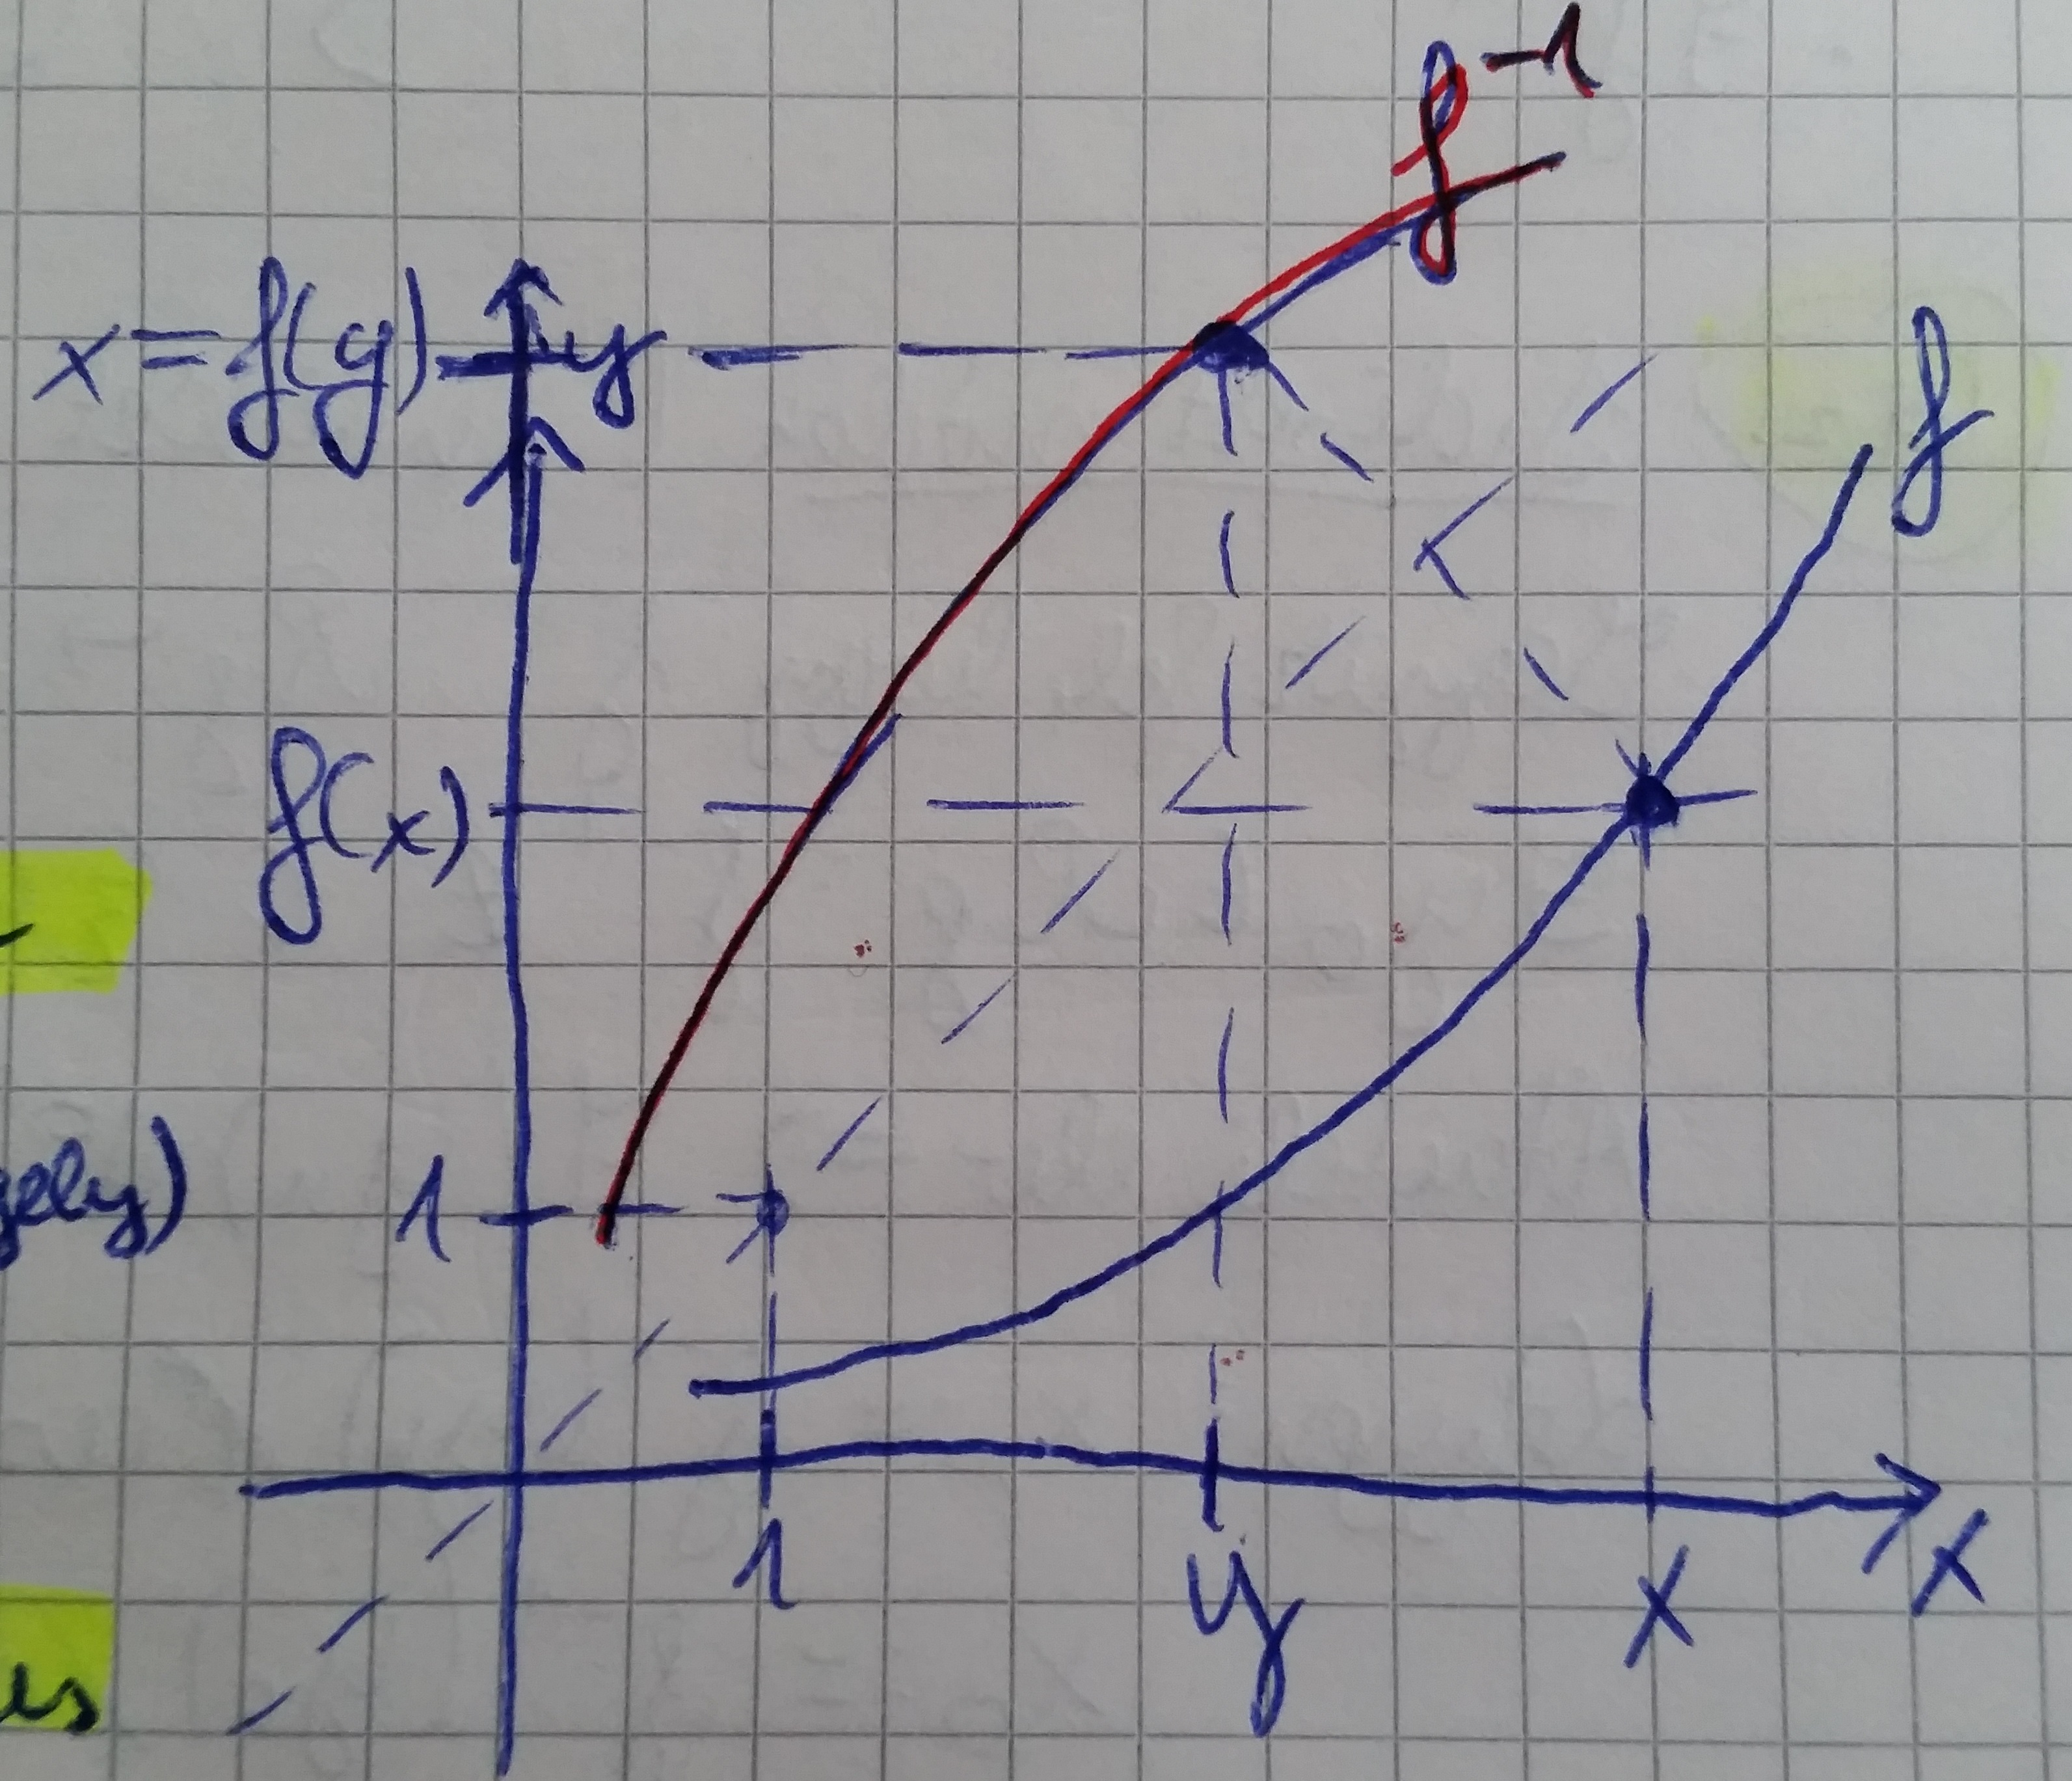
\includegraphics[height=3cm]{kepek/inverse_function.jpg}
		\caption{}\label{}
	\end{figure}
	\begin{theorem}
		(Az inverz függvény deriválása)
		
		Tegyük fel, hogy $f:(\alpha,\beta)\to\R$
		
		$\left.\begin{gathered}
			\text{szig. mon. és folytonos }
			(\alpha,\beta)\text{-n}\\
			\text{egy} a\in(\alpha,\beta)\text{-ban } f\in D\{a\}\\
			f'(a)\not=0 
		\end{gathered}\right\}\quad \Rightarrow\quad \begin{gathered}
		f\{-1\}\in D\{b\}, \text{ ahol } b:=f(a)\text{ és}\\
		(f^{-1})^{-1}(b)=\frac{1}{f'(a)}=\frac{1}{f'(f^{-1}(b))}
		\end{gathered}$
		\textit{Bizonyítás:} Csak szóbalin.\quad $\blacksquare$
	\end{theorem}
	\begin{note}
		$f:(\alpha,\beta)\to\R$ szig mon és folyt $(\alpha
		,\beta)$-n:
		
		Tegyük fel, hogy $f'(x)\not=0\quad \forall x\in(\alpha,\beta)$
		
		$(f(x)=y)\quad \Rightarrow\quad f^{-1}\quad $mindenütt deriválható
		\[ (f^{-1})'(y)=\frac{1}{f'(f^{-1}(y))}\quad (\forall y) \]
		\begin{center}
			\fbox{$\displaystyle (f^{-1})'=\frac{1}{f\circ f^{-1}}$}
		\end{center}
	\end{note}
	\begin{theorem}
		(Hatványsorok összegfüggvényének deriválása)
		
		Legyen $a\in\R,\quad \alpha_n\in\R(n=0,1,\ldots)$. Tegyük fel, hogy
		\[ \sum_{n=0}\alpha_n(x-a)^n\quad (x\in\R) \]
		hatványsor konvergenciasugara ($R$) pozitív.
		
		Legyen:
		\[ f(x):=\sum_{n=0}^{+\infty}\alpha_n(x-a)^n\quad (x\in K_R(a)) \]
		az összegfüggvény.
		
		Ekkor $\forall x\in K_R(a)$ esetén $f\in D\{x\}$, és 
		\[ f'(x)=\sum_{\fbox{$n=1$}}^{+\infty} n\alpha_n(x-a)^{n-1}\quad (x\in K_R(a)) \]
		\textit{Bizonyítás:} \textbf{NE LESZ KÉRDEZVE!}\quad $\blacksquare$
	\end{theorem}
	\begin{example}
		$\sin$ fv.
		\[ (\sin x)'= \left(x-\frac{x^3}{3!}+\frac{x^5}{5!}-\ldots\right)' = 1-\frac{x^2}{2!}+\frac{x^4}{4!}-\ldots=\cos x\quad \blacksquare \]
	\end{example}
	\section{Néhány elemi fv. deriváltja. (folytatás)}
	
	\begin{example}
		Polinomfüggvény: 
		\[ P(x)=a_nx^n+a_{n-1}x^{n-1}+\ldots+a_1x+a_0 \quad(a_n,\ldots a_n\in\R, \quad a_0\not=0) \]
		Ekkor:
		\[ \forall x\in\R:\quad P\in D\{a\}\text{\quad és}\quad  \]
		\[ P'(x)=na_nx^{n-1}+(n-1)a_{n-1}x^{n-2}+\ldots+a_1 \]
	\end{example}
	\begin{example}
		$\tan$ függvény:
		
		$\text{tg}:=\frac{\sin}{\cos};\quad \text{tg}x:=\text{tg}(x):=\frac{\sin x}{\cos x}$
		\[ \mathcal{D}_{\text{tg}}=\{ x\in\R\ | \ \cos x\not=0 \} \]
		Később jellemezzük.
		
		\medskip
		$\forall x\in\mathcal{D}_{\text{tg}}:\quad \text{tg}\in D\{x\}$ \quad és
		\[ \text{tg}'x=\left(\frac{\sin x}{\cos x}\right)=\frac{\sin'x\cos x-\sin x\cdot\cos'x}{\cos^2x}=\frac{1}{\cos^2x} \]
		\begin{center}
			\fbox{$\displaystyle \text{tg}'x=\frac{1}{\cos^2x}\quad (x\in\mathcal{D_{\text{tg}}})$}
		\end{center}
	\end{example}
	\begin{example}
		Kotangens fv.
		
		$\text{ctg}:=\frac{\cos}{\sin}$
		\begin{center}
			
			\fbox{$\displaystyle \text{ctg}'x=-\frac{1}{\sin^2x}\quad (x\in\mathcal{D}_{\text{tg}})$}
		\end{center}
	\end{example}
	\begin{example}
		Az $\exp$ függvény:
		
		$\forall x\in\R:\quad \exp\in D\{x\}$
		\[ \exp'x=\left(1+x+\frac{x^2}{2!}+\frac{x^3}{3!}+\ldots\right)'=1+x+\frac{x^2}{2!}+\frac{x^3}{3!} = \exp x \]
		\begin{center}
			\fbox{$\displaystyle (e^x)'=e^x\quad x\in\R$}
		\end{center}
		\begin{note}
			Deriváltja önmaga.
		\end{note}
	\end{example}
	\begin{example}
		Az $\ln$ függvény
		
		$\ln :=(\exp)^{-1}$
		\[ \forall x>0\quad \ln\in D\{x\}\quad \text{és} \]
		\begin{center}
			\fbox{$ \displaystyle \ln'x=\frac{1}{x}\quad (x\in(0,+\infty)) $}
		\end{center}
	\end{example}
	\begin{example}
		Az $\exp_a$ függvény: \quad $(a^x=e^{x\cdot\ln a})$
		$\forall x\in\R,\quad \exp_a\in D\{a\}$
		\begin{center}
			\fbox{$(a^x)'=a^x\ln a \quad (x\in\R)$}
		\end{center}
	\end{example}
	\begin{example}
		$\log_a$ függvény, $0<a$ és $a\not=1$
		
		\[ \forall c\in(0,+\infty),\quad \log_a\in D\{x\} \]
		\begin{center}
			\fbox{$\displaystyle \log_a'x=\frac{1}{x\cdot\ln a}\quad (x\in(0,+\infty))$}
		\end{center}
	\end{example}
	\begin{example}
		Hatványfüggvény:\quad $\alpha>0$
		$\displaystyle h_\alpha:=x^\alpha\quad (x\in(0,+\infty))$
		\[ \forall x>0, h_\alpha\in D\{x\} \quad \text{és} \]
		\begin{center}
			\fbox{$\displaystyle (x^\alpha)'=\alpha\cdot x^{\alpha-1}\quad (x\in(0,+\infty))$}
		\end{center}
	\end{example}
	\begin{example}
		{\Large WTF?!!}
	\end{example}
	\begin{example}
		Hiperbolikus függvények:
		th$:=\frac{\text{sh}}{\text{ch}}$ - tangenshiperbolikusz függvény
		
		cth$:=\frac{\text{ch}}{\text{sh}}$ - kotangenshiperbolikusz függvény.
	\end{example}
\end{document}
